\documentclass[spanish]{scrartcl}
\usepackage[spanish]{babel}
\selectlanguage{spanish}
\usepackage[utf8]{inputenc}
\usepackage{listings}
\usepackage{amsmath}
\usepackage[backend=biber]{biblatex}
\usepackage{graphicx}
\usepackage[usenames,dvipsnames]{color} % Required for specifying custom colors and referring to colors by name
\usepackage[colorlinks=true,linkcolor=blue,citecolor=blue,urlcolor=blue]{hyperref}

\lstset{language=Python, frame=single}
\let\endtitlepage\relax
\renewcommand{\and}{\vspace{1cm}}
\subtitle{Métodos Numéricos Avanzados}
\title{Speech Compression}
\author{
Juan Pablo Orsay - 49373 \\
Horacio Miguel Gomez - 50825 \\
Sebastián Andrés Maio - 50386 \\
Federico Bond - 52247 \\
Braulio Sespede - 51074
}
\date{Noviembre 2016}
\bibliography{informe}
\definecolor{DarkGreen}{rgb}{0.0,0.4,0.0} % Comment color
\definecolor{highlight}{RGB}{255,251,204} % Code highlight color

\lstdefinestyle{Style1}{ % Define a style for your code snippet, multiple definitions can be made if, for example, you wish to insert multiple code snippets using different programming languages into one document
language=Python, % Detects keywords, comments, strings, functions, etc for the language specified
basicstyle=\footnotesize\ttfamily, % The default font size and style of the code
breakatwhitespace=false, % If true, only allows line breaks at white space
breaklines=true, % Automatic line breaking (prevents code from protruding outside the box)
captionpos=b, % Sets the caption position: b for bottom; t for top
commentstyle=\usefont{T1}{pcr}{m}{sl}\color{DarkGreen}, % Style of comments within the code - dark green courier font
%deletekeywords={}, % If you want to delete any keywords from the current language separate them by commas
%escapeinside={\%}, % This allows you to escape to LaTeX using the character in the bracket
firstnumber=1, % Line numbers begin at line 1
frame=single, % Frame around the code box, value can be: none, leftline, topline, bottomline, lines, single, shadowbox
frameround=tttt, % Rounds the corners of the frame for the top left, top right, bottom left and bottom right positions
keywordstyle=\color{Blue}\textbf, % Functions are bold and blue
%morekeywords={}, % Add any functions no included by default here separated by commas
numbers=left, % Location of line numbers, can take the values of: none, left, right
numbersep=10pt, % Distance of line numbers from the code box
numberstyle=\tiny\color{Gray}, % Style used for line numbers
rulecolor=\color{black}, % Frame border color
showstringspaces=false, % Don't put marks in string spaces
showtabs=false, % Display tabs in the code as lines
stepnumber=1, % The step distance between line numbers, i.e. how often will lines be numbered
stringstyle=\color{Purple}, % Strings are purple
tabsize=2, % Number of spaces per tab in the code
}

\usepackage{subfig}
\usepackage[section]{placeins}

% Create a command to cleanly insert a snippet with the style above anywhere in the document
\newcommand{\insertcode}[2]{\begin{itemize}\item[]\lstinputlisting[caption=#2,label=#1,style=Style1]{#1}\end{itemize}} % The first argument is the script location/filename and the second is a caption for the listing

%----------------------------------------------------------------------------------------
\begin{document}
\maketitle
\endtitlepage

\begin{abstract}
En este trabajo implementaremos un simple compresor del habla. Nos basaremos en \textit{2nd International Conference on Computer and Communication Technology}, donde se propone un esquema muy simple de compresión basado en tres pasos: transformación, cuantificación y codificación Huffman.
\end{abstract}
\break
\tableofcontents
\break
\section{Procedimiento}
Para realizar la compresión seguimos los siguientes pasos:
\begin{enumerate}
\item Obtener la FFT de la muestra de audio.
\item De los coeficientes obtenidos se guarda la mitad +1.
\item Los coeficientes cuyo valor absoluto es menor que \textit{Epsilon} se los hace 0.
\item Cuantificamos la parte real y la imaginaria de los coeficientes con $L$ bits.
\item Codificamos con el algoritmo de Huffman los coeficientes.
\end{enumerate}
Para recuperar la grabación, hace falta de-codificar la información generada previamente y aplicar IFFT inversa.
\section{Ejemplo compresión y descompresión}
Para realizar la compresión y descompresión de un archivo de sonido, abrir octave dentro del directorio \textit{src} del proyecto y ejecutar lo siguiente:
\begin{lstlisting}
    wavName = "01"
    epsilon = 0.1
    L = 16
    [compressed, scale] = compress(wavName, epsilon, L)
\end{lstlisting}

Siendo:
\begin{enumerate}
    \item $wav_name$ el nombre del archivo dentro de resources/wav a comprimir
    \item $epsilon$ el valor a utilizar para eliminar ruido
    \item $L$ el número de bits a utilizar en la cuantización
\end{enumerate}
En \textit{compressed} obtenemos el wav comprimido, cuantizado y truncado que luego puede ser descomprimido mediante el siguiente código:
\begin{lstlisting}
    wav_name = "01" % 01_recompressed.wav
    uncompressed(compressed, "01")
\end{lstlisting}
\pagebreak
\section{Resultados}
Al ejecutar el código para comprimir y descomprimir el archivo \textit{11.wav}, obtuvimos los siguientes resultados.
\subsection{Compresión}

\begin{figure}[!htbp]
    \centering
    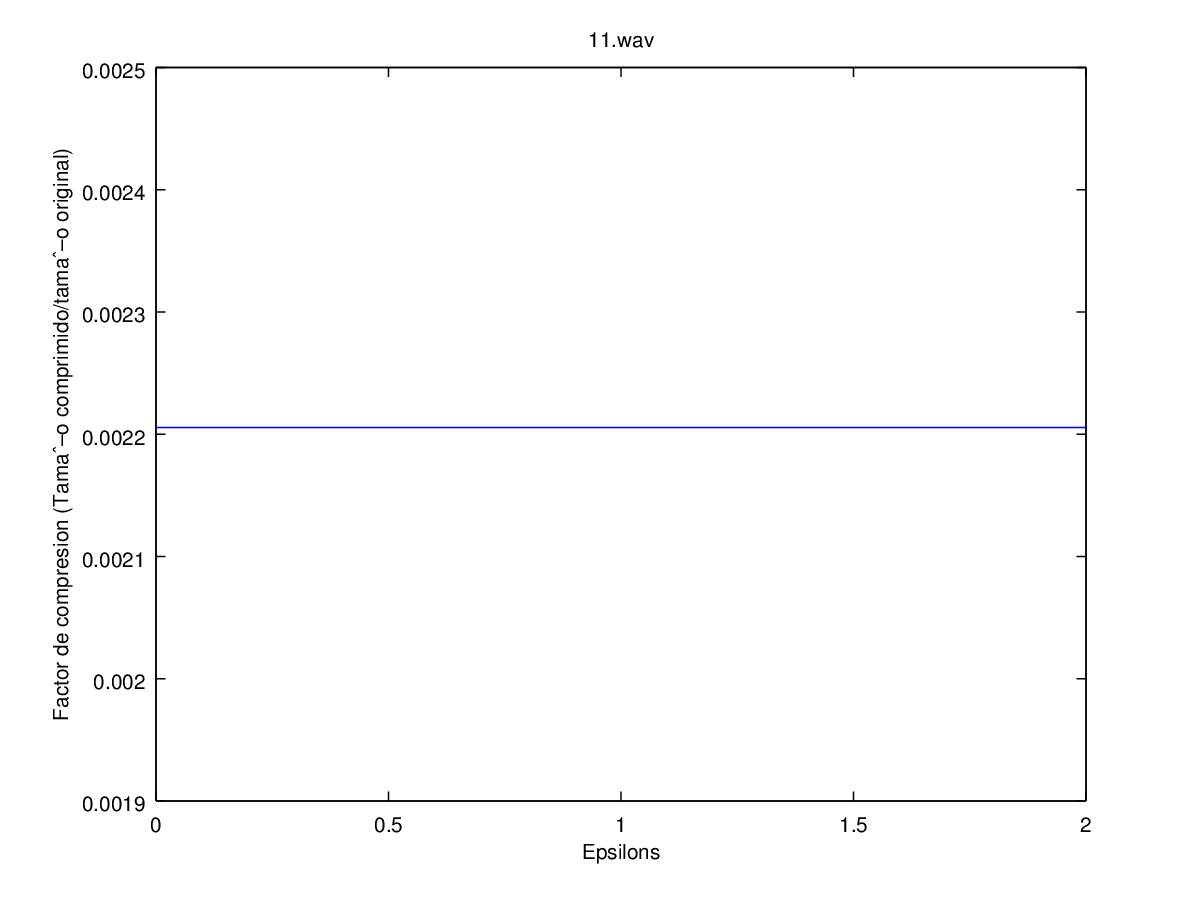
\includegraphics[interpolate=false, scale=0.65]{plots/11_epsi_compression}
    \caption{Factor de compresión}
    \label{fig:comp_fact}
\end{figure}

\pagebreak

\subsection{Relación entre bits mapeados y compresión}

\begin{figure}[!htbp]
    \centering
    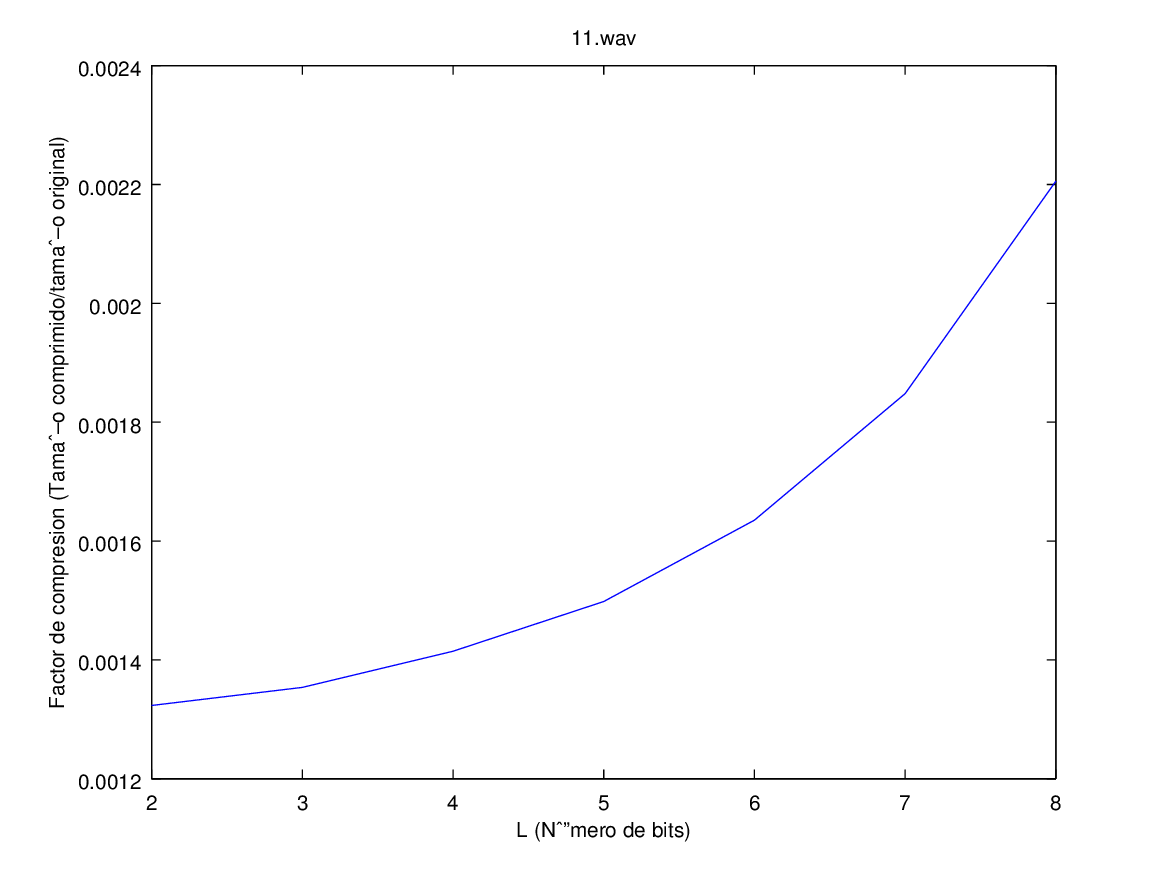
\includegraphics[interpolate=false, scale=0.65]{plots/11_bits_compression}
    \caption{Relación entre factor de compresión y bits utilizados para el mapeo}
    \label{fig:fact_bits}
\end{figure}

\pagebreak

\subsection{Distorsión cuadrática media}

\begin{figure}[!htbp]
    \centering
    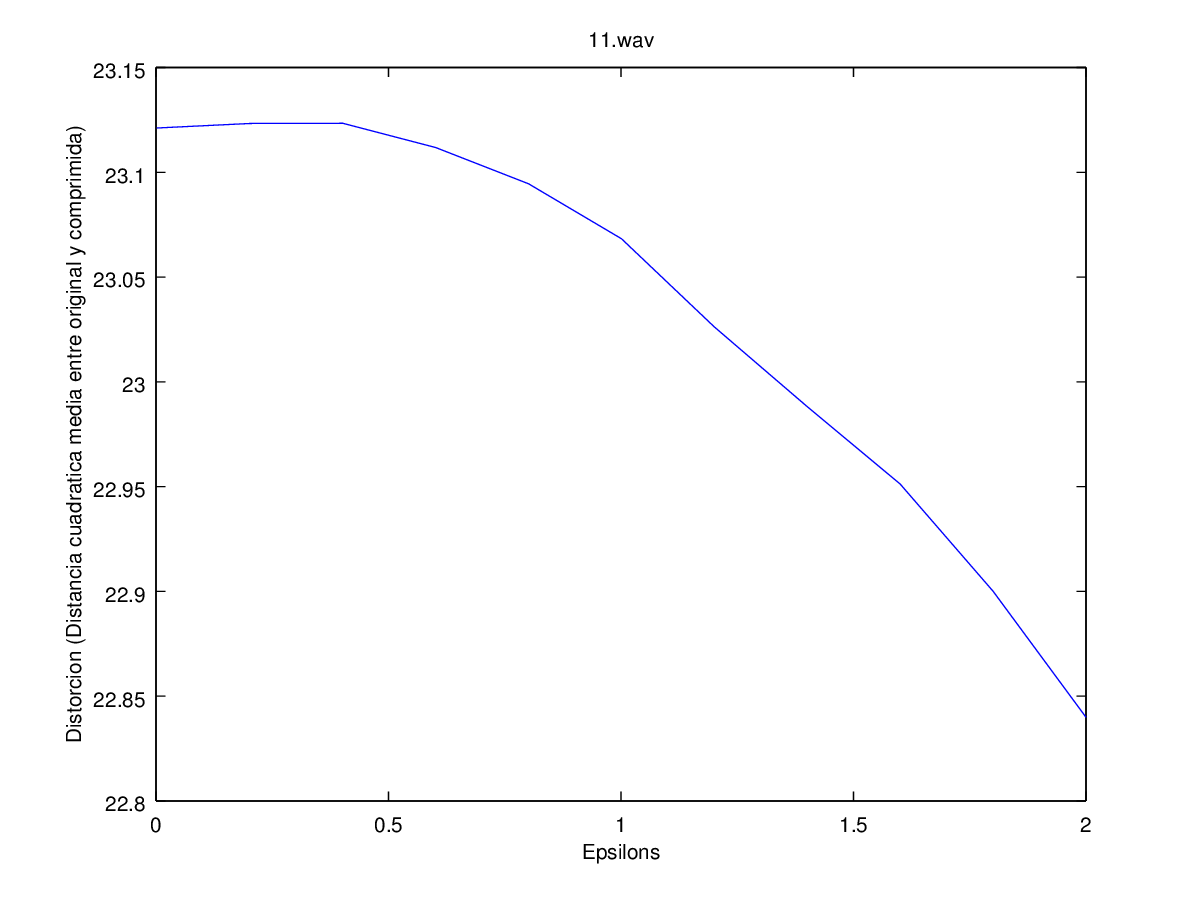
\includegraphics[interpolate=false, scale=0.65]{plots/11_epsi_distortion}
    \caption{Distorsión cuadrática media respecto de \textit{epsilon}}
    \label{fig:dist_epsi}
\end{figure}

\pagebreak

\subsection{Distorsión}

\begin{figure}[!htbp]
    \centering
    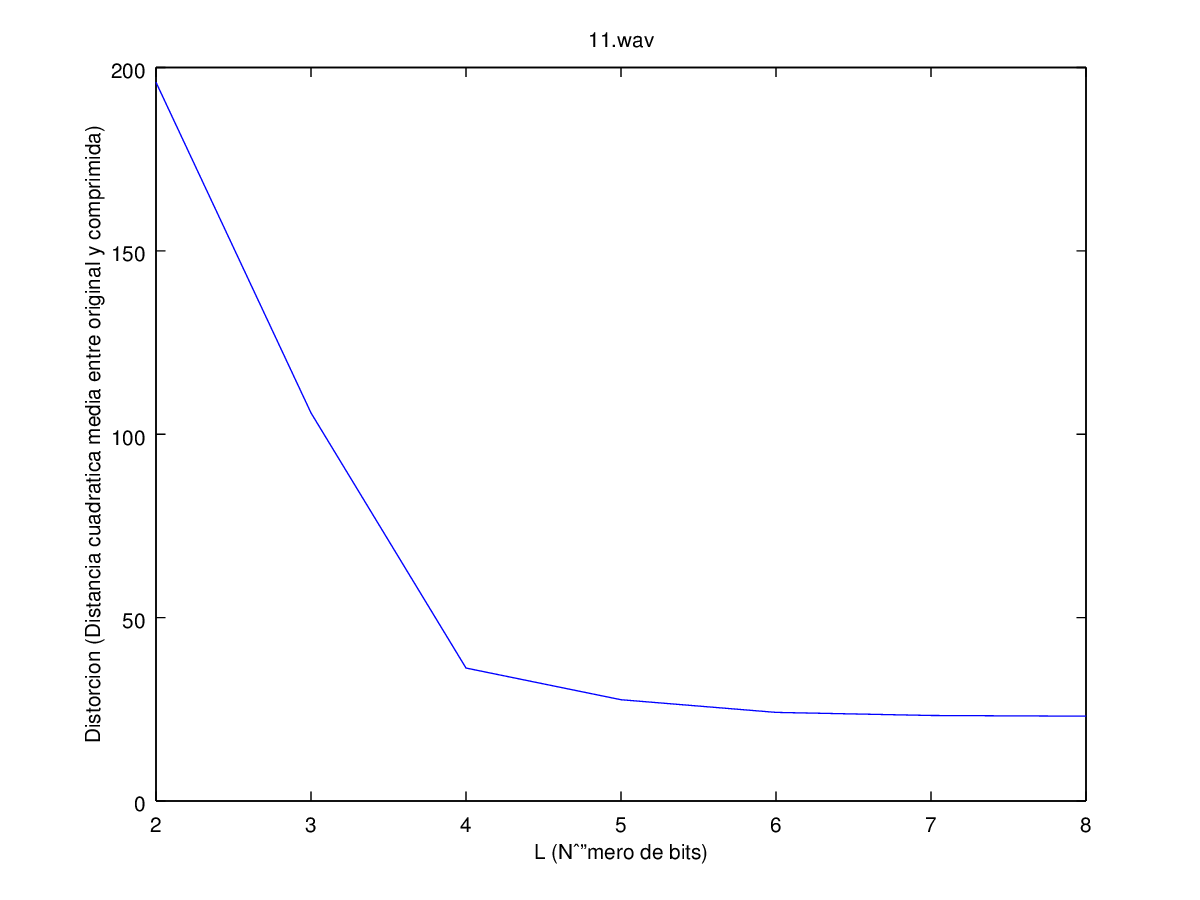
\includegraphics[interpolate=false, scale=0.65]{plots/11_bits_distortion}
    \caption{Distorcion cuadratica media respecto de la cantidad de bits utilizados}
    \label{fig:dist_bit}
\end{figure}

\pagebreak

\section{Conclusión}
Pudimos observar que cuantos menos bits utilizamos a la hora de cuantizar los coeficientes resultantes de la FFT de las muestras presentadas obtenemos un factor de compresión considerable pero, a su vez, encontramos que tras descomprimir lo obtenido previamente el sonido resultante tiene un gran número de ruido. \\
Por otro lado encontramos que a mayores números de épsilon, más apagado se escucha el audio descomprimido ya que al tener números altos de épsilon estamos filtrando una mayor amplitud del sonido resultando en la pérdida de contenido y definición. \\
Por último, encontramos que por alguna razón que desconocemos, todos los audios que comprimimos, al ser descomprimidos tienen una gran caída de volumen en el medio de la grabación. 

\section{Anexo}
\subsection{Código}
Dentro de la carpeta \textit{src} se encuentran los archivos de octave utilizados en la implementación del trabajo práctico:
\begin{itemize}
    \item compress.m: código para comprimir un archivo de sonido
    \item uncompress.m: código para descomprimir un archivo de sonido
    \item main.m: archivo que comprime y descomprime los archivos de prueba
    \item plot\_fixed\_bits.m: código para generar los gráficos
    \item plot\_fixed\_epsilon.m: código para generar los gráficos
    \item stats.m: código que genera estadísticas sobre la compresión/descompresión a ser utilizadas en los gráficos
    \item uncompress.m: código para descomprimir un archivo comprimido mediante el método propuesto
    \item huffman.m y myhuffmandict.m: código relacionado a la codificación huffman\cite{huffman}

\end{itemize}

\printbibliography

\end{document}
